\documentclass[a4paper,12pt,titlepage]{article}

\usepackage[german,ngerman]{babel}
\usepackage{fontspec}
\setmainfont{Calibri}
\usepackage{graphicx}
\usepackage{hyperref}
\usepackage{caption}
\usepackage{amsfonts}
\usepackage{amsmath}
\usepackage{listings}
\usepackage{xcolor}


\definecolor{dunkelblau}{RGB}{16, 55, 188}
\definecolor{orange}{RGB}{255, 60, 0}
\definecolor{gruen}{RGB}{18, 118, 34}
\definecolor{gelb}{RGB}{255, 200, 0}
\definecolor{lila}{RGB}{147, 18, 114}

\lstdefinestyle{code}{
language=c++,
 literate=
    {'}{{\textquotesingle}}1, % ' wird als Apostroph ausgegeben
commentstyle=\color{gruen}, 
keywordstyle =\color{black}, 
%Bis hier hin Farbgebung
frame=single, % Umrandung des Codes
rulecolor=\color{lightgray},
numbers=left, % Nummerierung hinzufügen (links)
numberstyle=\tiny, % Stil der Zeilennummern
stepnumber=1, % Schrittzahl für die Nummerierung
numbersep=5pt, % Abstand zwischen Nummerierung und Code
basicstyle=\sffamily, % Ändert die Schriftart des Codes
tabsize = 4, %Tab-Abstand
breaklines=true, %Zeilenumbruch
showstringspaces=false
}

\begin{document}

\begin{titlepage}
    \centering
    \vspace*{2cm}
    {\LARGE\bfseries Automaten und formale Sprachen Blatt 6\par}
    \vspace{2cm}
    {\Large Jan Lucca Agricola (275867) \& Jakob Schulz (275258)\par}
    \vspace{2cm}
    {\large\today\par}
\end{titlepage}

\section{Aufgabe}
\subsection{}
$f: \mathbb{Z} \times \mathbb{N}\textbackslash\{0\} \rightarrow \mathbb{N}$ mit: \\
$$f(m,n) =\left\{ \begin{array}{ll}\frac{1}{2}(2*m+n)\ast(2*m+n+1) + 2*m & \text{für } m \geq 0\\ \frac{1}{2}(-2*m-1+n)\ast(-2*m-1+n+1) -2*m-1 & \text{für } m < 0\end{array} \right.$$
\subsection{}
$f: \Sigma^* \rightarrow \mathbb{N}$ mit :\\
$w \in \Sigma^*$\\
$\Sigma' =$ Die Elemente von $\Sigma$ in lexikographischer Ordnung\\
Für jedes $b \in \Sigma$ den Rang von b in $\Sigma'$ (beginnend bei 1) mit  der Größe des Alphabets (\Sigma) hoch die Position von b in w (beginnend bei 0)\\
Addiere das Produkt zum Ergebnis.\\
Das leere Wort (\epsilon) hat 0 als Ergebnis\\
\\
\textbf{Beispiel}\\
$\Sigma = \{a, b, c\}$\\
\\
$f: \Sigma^* \rightarrow \mathbb{N}$\\
\begin{itemize}
\item $\epsilon \rightarrow 0$
\item $a \rightarrow 1*3^0$
\item $b \rightarrow 2*3^0$
\item $c \rightarrow 3*3^0$
\item $aa \rightarrow 1*3^1+1*3^0 = 4$
\item $ab \rightarrow 1*3^1+2*3^0 = 5$
\item $ac \rightarrow 1*3^1+3*3^0 = 6$
\item $ba \rightarrow 2*3^1+1*3^0 = 7$
\item ...
\end{itemize}


\subsection{}
Beweisskizze:\\
Angenommen die Menge der totalen Funktionen $f :  \mathbb{N} \rightarrow \{0,1\}$ wäre abzählbar. Hieraus folgt, dass es eine Aufzählung dieser Funktionen geben muss. Diese könnte schematisch wie folgt aussehen:\\
\\
\begin{tabular}{|c||c|c|c|c|c|c|}
\hline
&0&1&2&3&4&...\\
\hline
\hline
$f_0$&$f_0(0)$&$f_0(1)$&$f_0(2)$&$f_0(3)$&$f_0(4)$&...\\
\hline
$f_1$&$f_1(0)$&$f_1(1)$&$f_1(2)$&$f_1(3)$&$f_1(4)$&...\\
\hline
$f_2$&$f_2(0)$&$f_2(1)$&$f_2(2)$&$f_2(3)$&$f_2(4)$&...\\
\hline
$f_3$&$f_3(0)$&$f_3(1)$&$f_3(2)$&$f_3(3)$&$f_3(4)$&...\\
\hline
...&...&...&...&...&...&...\\
\hline
\end{tabular}
\\
\\
\\
Gemäß Annahme müssten in dieser Aufzählung alle Funktionen  $f :  \mathbb{N} \rightarrow \{0,1\}$ enthalten sein. Wir betrachten nun die Funktion $g:  \mathbb{N} \rightarrow \{0,1\}$, die wie folgt definiert wird:\\
\\
\begin{tabular}{|c||c|c|c|c|c|c|}
\hline
&0&1&2&3&4&...\\
\hline
\hline
$g$&$f_0(0)+1$&$f_1(1)+1$&$f_2(2)+1$&$f_3(3)+1$&$f_4(4)+1$&...\\
\hline
\end{tabular}\\
\\
\\
Die Funktion g wird in Abhängigkeit der Funktionen $f_0\text{, }f_1\text{, }f_2\text{, }f_3\text{, ...}$ definiert. 
Beispielsweise liefert die Funktion $g(0)$ den Wert $f_0(0)+1$. Dies bedeutet, dass die Funktion $g$ nicht identisch mit der Funktion $f_0$ ist, da sich der Funktionswert von $g$ und $f_0$ in dem Argument 0 unterscheidet. Mit analoger Begründung unterscheidet sich $g$ von den Funktionen $f_0\text{, }f_1\text{, }f_2\text{, }f_3\text{, ...}$ in den weiteren Argumenten. Das bedeutet, dass die Funktion $g$ nicht in der Aufzählung vorkommen kann. Dies ist jedoch ein Widerspruch zur Annahme, dass die Aufzählung alle Funktionen $g: \mathbb{N} \rightarrow \{0,1\}$ enthält.
Die Menge aller Funktionen $f: \mathbb{N} \rightarrow \{0,1\}$ ist überabzählbar.
\section{Aufgabe}
\subsection{}
\begin{lstlisting}[style = code]
whilenot iszero(A) do
	pred(A);
od;
succ(A);
succ(A);
succ(A);
succ(A);
succ(A);
\end{lstlisting}
\subsection{}
\begin{lstlisting}[style = code]
whilenot iszero(B) do
	succ(A);
	pred(B);
od;
\end{lstlisting}
\subsection{}
\begin{lstlisting}[style = code]
whilenot iszero(A) do
	succ(B);
	succ(C);
	pred(A);
od;
whilenot iszero(C) do
	succ(A);
	pred(C);
od;
\end{lstlisting}
\subsection{}
Annahme, dass A nicht negativ sein kann, also entweder 0 oder positiv
\begin{lstlisting}[style = code]
whilenot iszero(C) do
	pred(C);
od;
whilenot iszero(A) do
	whilenot iszero(C) do
		pred(C);
	od;
	succ(C);
	pred(A);
od;
\end{lstlisting}
\subsection{}
\begin{lstlisting}[style = code]
whilenot iszero(C) do
	pred(C);
od;
succ(C); //C auf 1 setzen

succ(B); //damit C auch 0 ist, wenn A = B
//A auf 0 setzen, B verringern
whilenot iszero(A) do
	pred(B);
	pred(A);
od;

//Wenn B ungleich 0 ist, dann ist B >= A
whilenot iszero(B) do
	pred(C);
	pred(A);
od;
\end{lstlisting}
\section{Aufgabe}
\subsection{}
\begin{lstlisting}[style = code]
whilenot iszero(B) do
	pred(A);
	pred(B);
od;
\end{lstlisting}
\subsection{}
\begin{lstlisting}[style = code]
//C und D auf 0 setzen
whilenot iszero(C) do
	pred(C);
od;
whilenot iszero(D) do
	pred(D);
od;

//Wert von A in C und C kopieren
whilenot iszero(A) do
	succ(C);
	succ(D);
	pred(A);
od;

//Für jedes B addieren den Wert von C auf A
whilenot iszero(B) do
	whilenot iszero(C) do
		succ(A);
		succ(D);
		pred(C);
	od;

	whilenot iszero(D) do
		succ(C);
	od;
	pred(B);
od;
\end{lstlisting}
\subsection{}
\begin{lstlisting}[style = code]
//Register C, D, E, F, G auf 0 setzen
whilenot iszero(C) do
	pred(C);
od;
whilenot iszero(D) do
	pred(D);
od;
whilenot iszero(E) do
	pred(E);
od;
whilenot iszero(F) do
	pred(F);
od;
whilenot iszero(G) do
	pred(G);
od;

//Register D und E den Wert von Register A zuweisen
whilenot iszero(A) do
	succ(D);
	succ(E);
	pred(A);
od;

//Register F und G den Wert von Register B zuweisen
wilenot iszero(B) do
	succ(F);
	succ(G);
	pred(B);
od;

//Register F um D reduzieren
whilenot iszero(D) do
	pred(F);
	pred(A);
od;

//Wenn F den Wert 0 hat ist B entweder kleiner oder gleich A
if iszero(F) then
	//Register E um den Wert G reduzieren
	wilenot iszero(G) do
		pred(E);
		pred(G);
	od;

	//Wenn Register G den Wert 0 hat muss gelten A = B
	if iszero(G) do
		succ(C);
	od;
fi;
\end{lstlisting}
\subsection{}
\begin{lstlisting}[style = code]//Register C, D, E, F, G auf 0 setzen
whilenot iszero(C) do
	pred(C);
od;
whilenot iszero(D) do
	pred(D);
od;
whilenot iszero(E) do
	pred(E);
od;
whilenot iszero(F) do
	pred(F);
od;
whilenot iszero(G) do
	pred(G);
od;

//Register D und E den Wert von Register A zuweisen
whilenot iszero(A) do
	succ(D);
	succ(E);
	pred(A);
od;

//Register F und G den Wert von Register B zuweisen
wilenot iszero(B) do
	succ(F);
	succ(G);
	pred(B);
od;

//Register F um D reduzieren
whilenot iszero(D) do
	pred(F);
	pred(A);
od;

//Wenn F den Wert 0 hat ist A entweder groesser oder gleich B
if iszero(F) then:
		//Den Wert im Register G (B) von Register E (A) abziehen
		whilenot iszero(G) do
			pred(E);
			pred(G);
		od;
		//Das Ergebnis von E - G (A - B) in C schreiben
		whilenot iszero(E) do
			succ(C);
		od;
	else
		//Den Wert im Register E (B) von Register G (B) abziehen
		whilenot iszero(E) do
			pred(G);
			pred(E);
		od;
		//Das Ergebnis von G - E (B - A) in C schreiben
		whilenot iszero(G) do
			succ(C);
		od;
fi;
\end{lstlisting}
%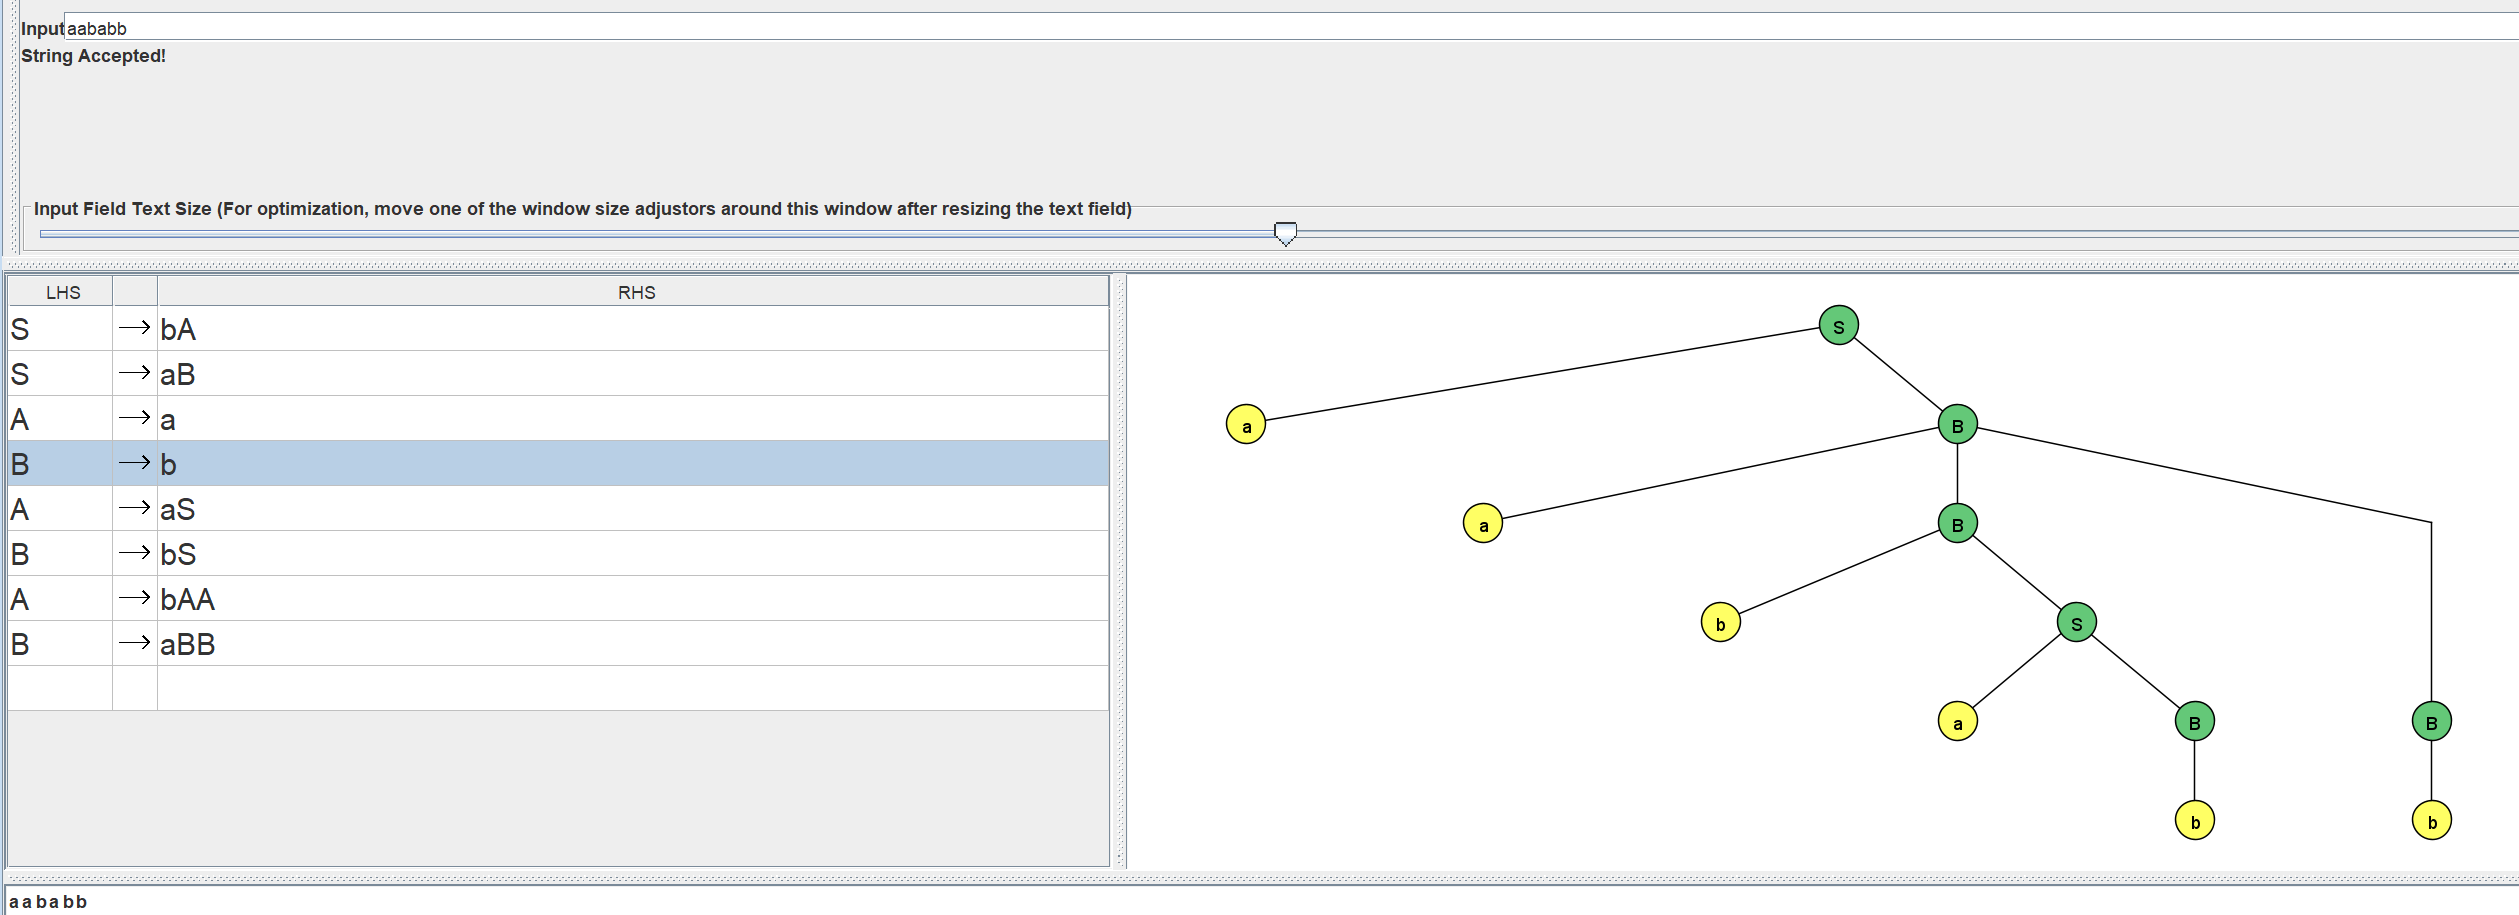
\includegraphics[width=1.0\textwidth]{syntaxtree_task9_4.png}\\
\end{document}
